% Appendix A

\chapter{Orthogonale Polynome im Askey Schema} % Main appendix title

\label{AppendixA} % For referencing this appendix elsewhere, use \ref{AppendixA}

\section{Geschichtliche Entstehung}
Die Entstehung des \emph{general Polynomial Chaos}(gPC) ist eine Geschichte über den Versuch, stochastische Abhängigkeit und Integrationstheorie zu kombinieren. Sie wurzelte in der Arbeit von Wiener (\autocite{norbertwiener1938}), wo er das \emph{homogene Chaos} einführte, um die Entwicklung von Unsicherheit in einem dynamischen, chaotischen, physikalischen System zu konkretisieren. Dies erklärt auch den Ursprung der Bezeichnung "`Chaos"' im Kontext der chaotischen Brownschen Bewegung im Wiener-Prozess.\\
Ghanem verwendete dann Hermite Polynome um mithilfe dieser Orthogonalbasis gaußsche Prozesse darzustellen. Dies wendete er erfolgreich auf einige Probleme aus den Ingenieurswissenschaften an, ein Überblick wird in \autocite{GhaSpa91} gegeben.\\
Xiu verallgemeinerte in seiner Arbeit \autocite{xiu2002} diesen Ansatz auf andere Kombinationen aus stochastischer Verteilung und Polynombasis. Gemäß dem Askey Schema (siehe Abbildung \ref{askeyscheme}) werden Beziehungen einiger bekannter Polynom Orthonormalbasen verdeutlicht. Man beobachtet außerdem, dass einige Gewichte den Dichtefunktionen von bekannten Verteilungen entsprechen und möchte nun zu einer gegebenen Verteilung die bestmögliche Polynombasis verwenden. An Modellproblemen demonstrierte Xiu jeweils optimale exponentielle Konvergenz für die verschiedenen Paarungen.\\
\begin{figure}
\center
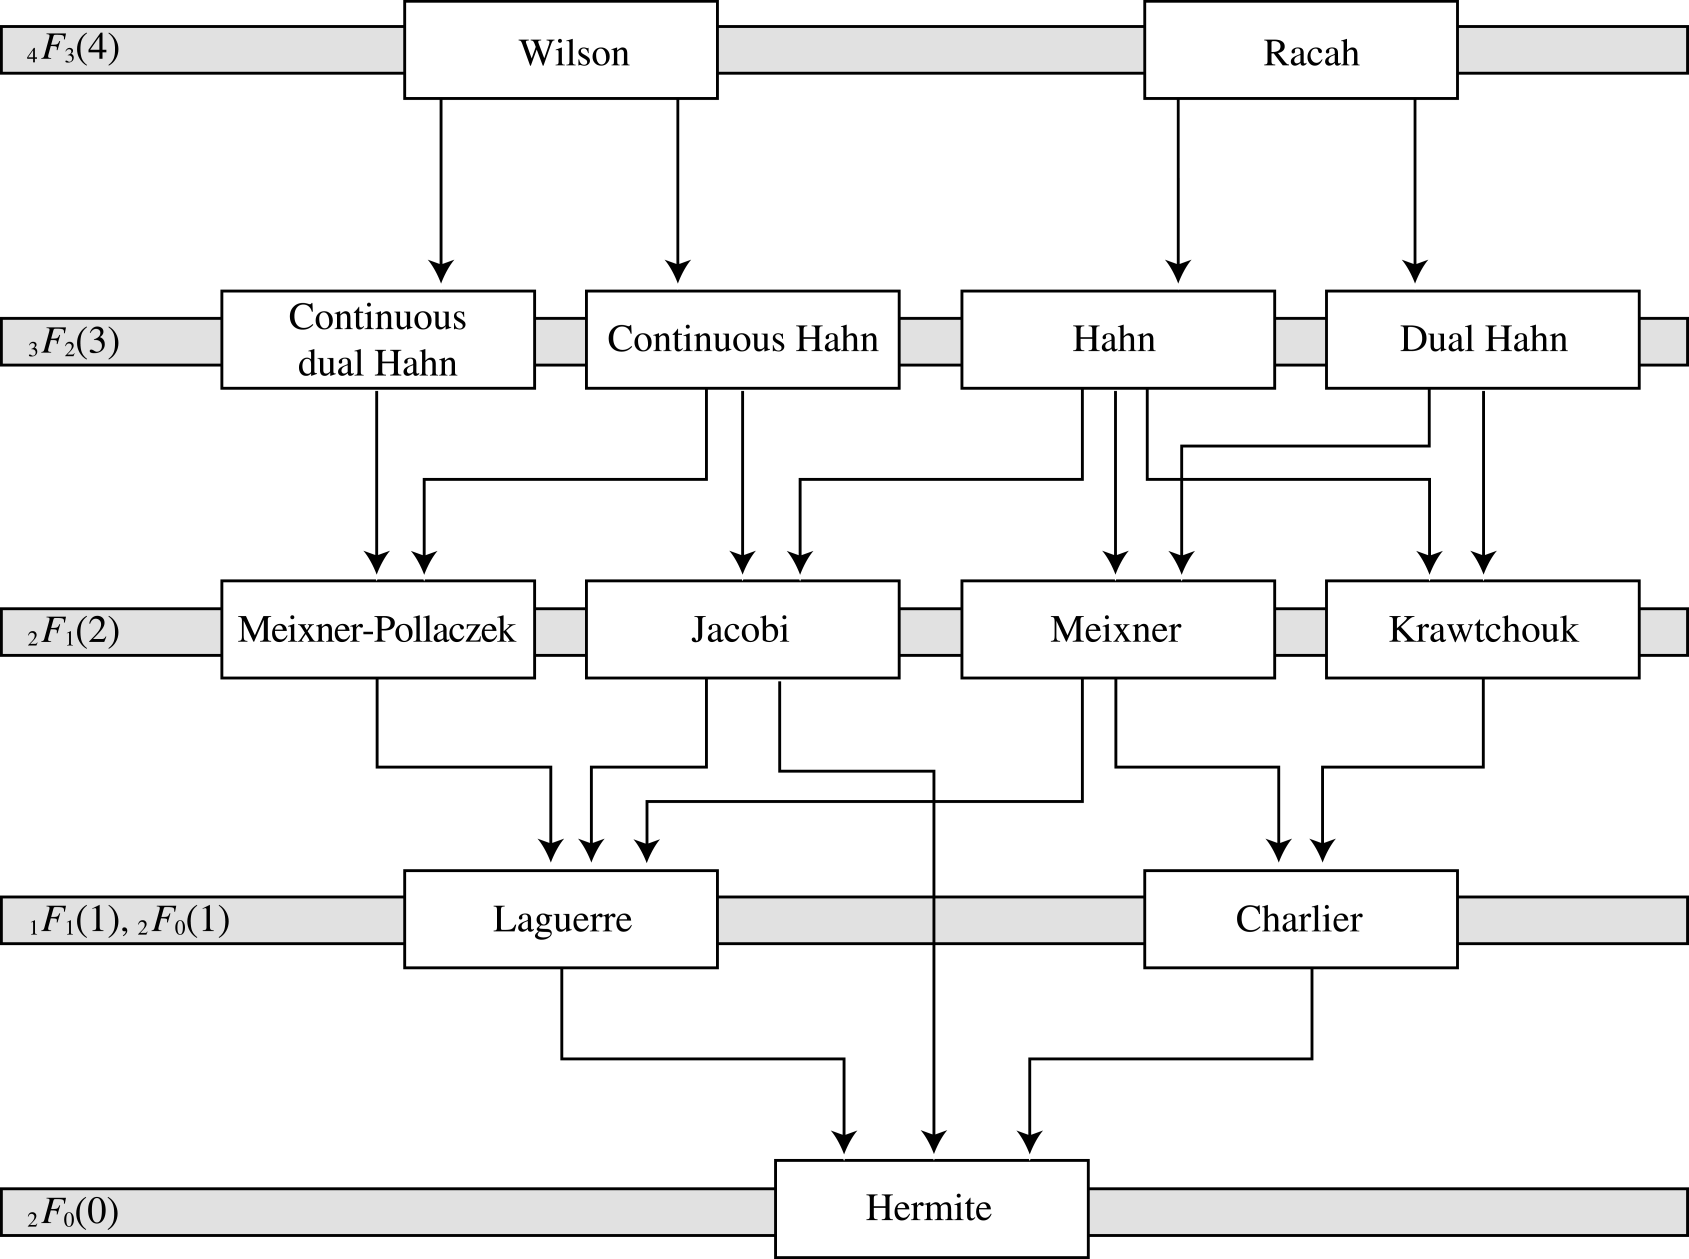
\includegraphics[width=0.8\linewidth]{Figures/askeyscheme.png}
\caption{Askey Schema; Ein Pfeil symbolisiert den Übergang einer Basis in eine andere durch Grenzwertbildung eines Parameters; Quelle: \autocite{webaskey}}
\label{askeyscheme}
\end{figure}
\begin{mathbsp}[Grenzwertbildung im Askey Schema]
Es gilt für die Jacobi Polynome $P_n^{(\alpha,\beta)}(x)$ und die Hermite Polynome $H_n(x)$ die Beziehung
\[\lim\limits_{\alpha\to\infty}\alpha^{-\onehalf n}P_n^{(\alpha,\alpha)}\left(\frac{x}{\sqrt{\alpha}}\right)=\frac{H_n(x)}{2^nn!}\]
Für eine genauere Betrachtung der Beziehungen der hypergeometrischen Polynome im Askey Schema sei auf \autocite{koekoekswart98} verwiesen.
\end{mathbsp}

\section{Auflisting von Polynombasen und Verteilungen}
Wir präsentieren hier eine Auswahl der von uns verwendeten Orthogonalpolynome, insbesondere ihre Definition, Darstellung als Drei Term Rekursion, Gewichtsfunktion und ihre Beziehung zu stochastischen Verteilungen. Für weitere Eigenschaften wie die Darstellung als Lösung einer Differentialgleichung oder die Rodriguez Formel sei beispielsweise auf den Anhang von \autocite{dongbinxiu2010} verwiesen.\\
Eine schöne Übersichtstabelle findet sich unter \url{http://dlmf.nist.gov/18.3}, man beachte, dass dort die verwendeten Polynome und Gewichte teilweise von unserer Notation abweichen. Dies ist der Tatsache geschuldet, dass die Beziehung zu Verteilungen und entsprechende Normierungsanforderungen keine Rolle spielen. Ebenso gibt es verschiedene Varianten die untere Grenze für die Parameter $\alpha$ und $\beta$ der Jacobi und Laguerre Polynome zu definieren.\\
Benötigt man Referenzwerte für Nullstellen und Gewichte einer zugehörigen Gauss Quadratur, so findet sich unter\\\url{http://keisan.casio.com/exec/system/1281279441} ein Onlinerechner.\\
Hierbei sei wieder auf abweichende Notation hingewiesen, insbesondere die fehlende Normierung der Gewichte um einen Faktor.\\
Um die Polynome möglichst kompakt darzustellen zu können, werden folgende Definitionen nützlich sein.
\begin{mathdef}[Pochhammer Symbol]
Das Pochhammer Symbol $(a)_n$ für $a\in\R$ und $n\in\lbrace -1,0,1,2,\dots\rbrace$ sei definiert durch
\[(a)_n=
   \begin{cases}
   1, &n=-1\text{ oder } n=0\\
   a(a+1)\dots (a+n-1), &n\in\N
   \end{cases}\left(\stackrel{n\in\N}{=}\frac{\Gamma(a+n)}{\Gamma(a)}\right)
   \]
Beachte, dass dies auch \emph{steigende Fakultät} genannt wird und nicht mit der \emph{fallenden Fakultät} verwechselt werden sollte, wie das Symbol auch manchmal verwendet wird. Die Notation ist in der Literatur nicht einheitlich!
\end{mathdef}

\begin{mathdef}[Hypergeometrische Funktion]
Zu $r,s\in\N_0$ ist die hypergeometrische Funktion $_rF_s$ definiert durch
\[_rF_s(a_1,\dots,a_r;b_1,\dots,b_s;z)\coloneqq \sum_{k=0}^\infty \frac{(a_1)_k\dots (a_r)_kz^k}{(b_1)_k\dots(b_s)_kk!}\]
\end{mathdef}
Für weitere Polynome aus dem Askey Schema (siehe Abbildung \ref{askeyscheme}), insbesondere diese mit diskreten Verteilungen, sei wieder beispielsweise auf \autocite{dongbinxiu2010} verwiesen. \\
Für eine Methode zum Berechnen der Nullstellen aus der Drei-Term-Rekursion steht der Golub-Welsch-Algorithmus (vgl. \ref{golubwelschalg}) zur Verfügung.\\
Für die Drei-Term-Rekursion der nicht normalisierten orthogonalen Polynome $\Psi_n$ gilt stets $\Psi_{-1}\equiv 0$ und $\Psi_{0}\equiv 1$.
\subsection{Hermite Polynome und Gauß Verteilung}
Träger:
\[I=\R\]
Definition:
\[H_n(x)=(2x)^n\cdot {_2F_0}\left(-\frac{n}{2},-\frac{n-1}{2};\, ;-\frac{2}{x^2}\right)\]
Drei-Term-Rekursion:
\[H_{n}(x)=xH_{n-1}(x)-(n-1)H_{n-2}(x)\]
Gewichtsfunktion:
\[w(x)=\frac{1}{\sqrt{2\pi}}e^{-\frac{x^2}{2}}\]
Normalisierungsfaktor:
\[\gamma_n=n!\]
Stochastische Verteilung $\mathcal{N}(0,1)$:
\begin{center}
normalisierte Gauß Verteilung mit Dichtefunktion $\rho(x)=w(x)$
\end{center}

\subsection{Laguerre Polynome und Gamma Verteilung}
Träger:
\[I=(0,\infty)\]
Definition:
\[L_n^{(\alpha)}(x)=\frac{(\alpha)_n}{n!}\cdot {_1F_0}\left(-n;\alpha;x\right),\quad \alpha>0\]
Drei-Term-Rekursion:
\[L_{n}^{(\alpha)}(x)=\frac{2n-2+\alpha -x}{n}L_{n-1}^{(\alpha)}(x)-\frac{n-1+\alpha - 1}{n}L_{n-2}^{(\alpha)}(x)\]
Gewichtsfunktion:
\[w(x)=\frac{x^{\alpha-1}e^{-x}}{\Gamma(\alpha)}\]
Normalisierungsfaktor:
\[\gamma_n=\frac{(\alpha)_n}{n!}\]
Stochastische Verteilung $\gamma(\alpha,1)$:
\begin{center}
Gamma Verteilung mit $\alpha>0,\beta=1$ und Dichtefunktion
\[\rho(x)=\frac{x^{\alpha-1}e^{-\frac{x}{\beta}}}{\beta^{\alpha}\Gamma(\alpha)}\]
\end{center}

\subsection{Jacobi Polynome und Beta Verteilung}
Träger:
\[I=(-1,1)\]
Definition:
\[P_n^{(\alpha, \beta)}(x)=\frac{(\alpha + 1)_n}{n!}\cdot {_2F_1}\left(-n,n+\alpha+\beta+1;\alpha+1;\frac{1-x}{2}\right),\quad \alpha,\beta>-1\]
Drei-Term-Rekursion:
\begin{center}
Zum Abkürzen sei für $n\in\N\quad f_n \coloneqq \frac{(2n + \alpha + \beta - 1)(2n + \alpha + \beta)}{2n(n + \alpha + \beta)}$
\begin{align*}
P_n^{(\alpha, \beta)}(x)&=\left(f_nx-\frac{f_n(\beta^2-\alpha^2)}{(2n + \alpha + \beta - 2)(2n + \alpha +\beta)}\right)P_{n-1}^{(\alpha, \beta)}(x)\\
&\quad-\frac{2f_n(n + \alpha - 1)(n + \beta - 1)}{(2n + \alpha + \beta - 2)(2n + \alpha + \beta - 1)}P_{n-2}^{(\alpha, \beta)}(x)
\end{align*}
Man beachte, dass dies einige Definitionslücken aufweist:
\begin{itemize}
\item Für $\alpha=\beta=0$ stimmen die Jacobi Polynome exakt mit den Legendre Polynomen überein und die Betaverteilung mit der Gleichverteilung (siehe \ref{seclegendre}).
\item Für $\alpha+\beta=0,n=1$ gilt $P_1^{(\alpha,\beta)}(x)=x-\frac{\beta-\alpha}{2}$
\item Für $\alpha+\beta=-1,n=1$ gilt $P_1^{(\alpha,\beta)}(x)=\frac{x}{2}-\frac{\beta-\alpha}{2}$
\end{itemize}
\end{center}
Gewichtsfunktion:
\[w(x)=\frac{\Gamma(\alpha+\beta+2)}{2^{\alpha+\beta+1}\Gamma(\alpha+1)\Gamma(\beta+1)}(1-x)^\alpha(1+x)^\beta\]
Normalisierungsfaktor:
\[\gamma_n=\frac{(\alpha+1)_n(\beta+1)_n}{n!(2n+\alpha+\beta+1)(\alpha+\beta+2)_{n-1}}\]
Stochastische Verteilung $Beta(\alpha,\beta)$:
\begin{center}
Beta Verteilung auf $(-1,1)$ mit $\alpha,\beta>-1$ und Dichtefunktion
\[\rho(x)=\frac{(1 - x)^\alpha(1 + x)^\beta}{2^{\alpha + \beta + 1}B(\alpha+1,\beta+1)}=w(x),\quad B\text{ ist Eulersche Betafunktion}\]
\end{center}

\subsection{Legendre Polynome und Gleichverteilung}
\label{seclegendre}
Als wichtiger Spezialfall der Jacobi Polynome seien die Legendre Polynome an dieser Stelle explizit erwähnt.\\
Träger:
\[I=[-1,1]\]
Definition:
\[L_n(x)={_2F_1}\left(-n,n+1;1;\frac{1-x}{2}\right)\]
Drei-Term-Rekursion:
\[L_{n}(x)=x\frac{2n-1}{n}L_{n-1}(x)-\frac{n-1}{n}L_{n-2}(x)\]
Gewichtsfunktion:
\[w(x)\equiv \onehalf\]
Normalisierungsfaktor:
\[\gamma_n=\frac{1}{2n+1}\]
Stochastische Verteilung $\mathcal{U}(-1,1)$:
\begin{center}
Gleichverteilung auf $[-1,1]$ mit Dichtefunktion $\rho(x)=w(x)$
\end{center}
